\documentclass[norsk, a4paper]{article}

\usepackage[T1]{fontenc}    % Riktig fontencoding
\usepackage[utf8]{inputenc} % Riktig tegnsett
\usepackage{babel}          % Ordelingsregler, osv
\usepackage{graphicx}       % Inkludere bilder
\usepackage{booktabs}       % Ordentlige tabeller
\usepackage{url}            % Skrive url-er
\usepackage{textcomp}       % Den greske bokstaven micro i text-mode
\usepackage{units}          % Skrive enheter riktig
\usepackage{float}          % Figurer dukker opp der du ber om
\usepackage{lipsum}         % Blindtekst
\usepackage{amsmath}        % math

% JF i margen
\makeatletter
\renewcommand{\subsubsection}{\@startsection{subsubsection}{3}{-2cm}%
{-\baselineskip}{0.5\baselineskip}{\bf\large}}
\makeatother
\newcommand{\jf}[1]{\subsubsection*{JF #1}\vspace*{-2\baselineskip}}

% Skru av seksjonsnummerering
\setcounter{secnumdepth}{-1}

\begin{document}

% Forside
\begin{titlepage}
\begin{center}

\textsc{\Large FYS3220 - Lineær kretselektronikk}\\[0.5cm]
\rule{\linewidth}{0.5mm} \\[0.4cm]
{ \huge \bfseries  LABORATORIEØVELSE A}\\[0.10cm]
\rule{\linewidth}{0.5mm} \\[1.5cm]

\textsc{\Large Fourieranalyse}\\[1.5cm]

% Av hvem?
\begin{minipage}{0.49\textwidth}
    \begin{center} \large
        Snorre Bjørnstad (snorrebj)\\ \url{snorrebj@student.matnat.uio.no} \\[0.8cm]
        
\includegraphics[width = 0.5\textwidth ]{Figurer/snorre.jpg}
    \end{center}
\end{minipage}
\begin{minipage}{0.49\textwidth}
    \begin{center} \large
        Arne Johan Bergli (ajbergli)\\ \url{ajbergli@student.matnat.uio.no} \\[0.8cm]
        %\includegraphics{bilde2}
    \end{center}
\end{minipage}

\vfill

% Litt info nederst
\large{
\begin{tabular}{r@{: }l}
Labdag & XX \\
Dato & \today
\end{tabular}
}

\end{center}
\end{titlepage}

\section{Oppgave 1: Summering av signaler}
\jf{1.a}
\begin{figure}
 \begin{center}
   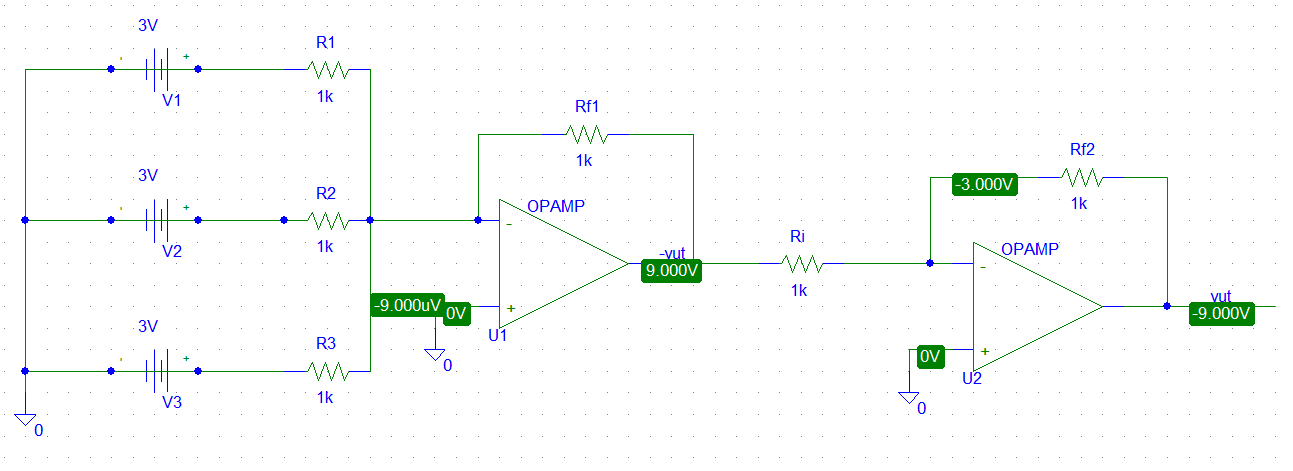
\includegraphics[width=1\textwidth]{Figurer/oppg1_schem.PNG}\\
   \caption{\textit{Summeringskretsen for oppgave 1a}}\label{fig:oppg1_schem}
 \end{center}
\end{figure}

Summeringskretsen vår er vist i figur \ref{fig:oppg1_schem}. Vi har altså 3 parallellkoblede batterier som alle går inn i en summeringskrets laget av to opamper med invers feedback. Som figuren viser er spenningen \(v_{ut}\) på  \(9 \unit{V}\) som forventet. 


\section{Oppgave 2: Simulering av egen blanding av frekvenskomponenter}
\jf{2.a}

\begin{align*}  v(t)&=0\\ &+ 1\cdot\sin{(2\pi\cdot 500Hz)}\\ &+ 0.5 \cdot \sin{(2\pi\cdot 1000Hz)}\\ &+ 0.6 \cdot \sin{(2\pi\cdot 1300Hz)}\\ &+ 0.4 \cdot \sin{(2\pi\cdot 1900Hz)}\\ & + 0.2 \cdot \sin{(2\pi\cdot 3000Hz)}
\end{align*}
 
\jf{2.b}
\begin{figure}
  \begin{center}
     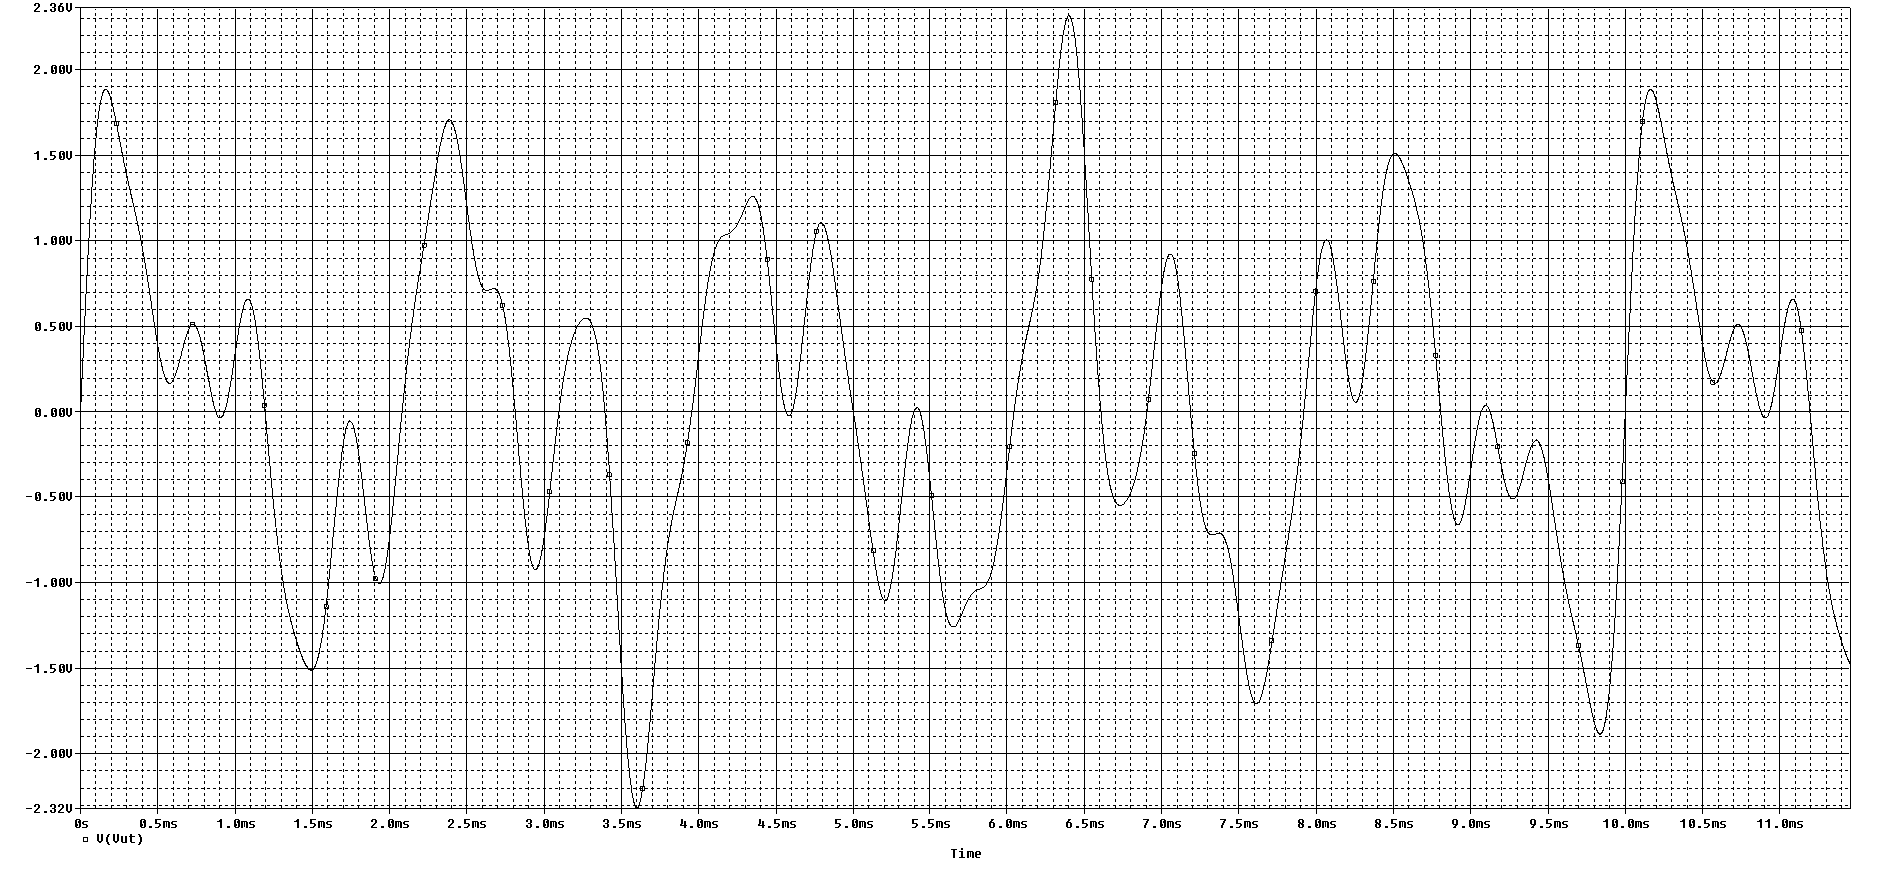
\includegraphics[width= 1\textwidth]{Figurer/oppg2_tid.png}
     \caption{Spenning tidsplott for Signalet Sumut med parameterene i Oppgave 2.a}\label{fig:oppg2_tid}
  \end{center}
\end{figure}
Se figur \ref{fig:oppg2_tid}
\jf{2.c}
 

\begin{figure}
  \begin{center}
      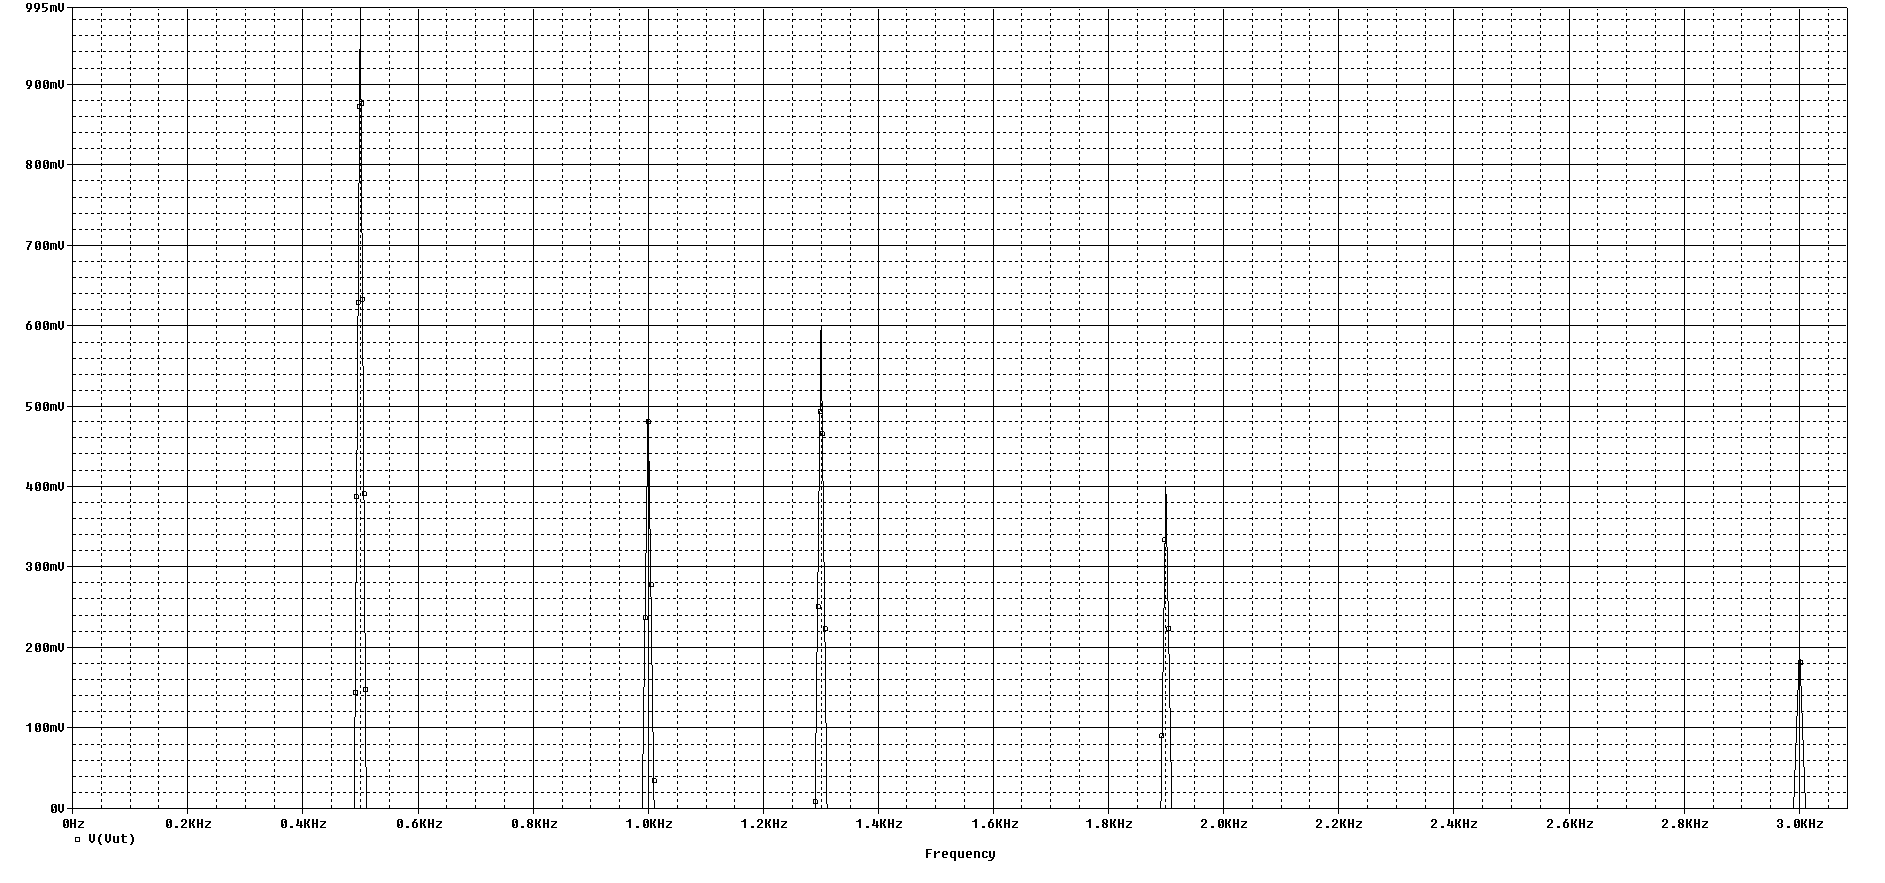
\includegraphics[width= 1\textwidth]{Figurer/oppg2_fft.png}
       \caption{Frekvenspekteret til signalet i Figur \ref{fig:oppg2_tid}. }\label{fig:oppg2_fft}
  \end{center}
\end{figure}

Frekvensspekteret til signalet vi genererte er vist i Figur \ref{fig:oppg2_fft}. Vi ser her hvilke frekvenser det totale signalet består av. Vi ser at hver av toppene i frekvensspekteret korresponderer til hvert sitt ledd i funksjonen i Oppgave 2.a
\section{Oppgave 3: dc og $b_n$ for $v(t)$}
\jf{3.a}
Utregning av \(dc\)-verdier:

\begin{align*}
dc &= \frac{1}{T} \int\limits_{0}^{\frac{T}{2}} 1 dt \\
&= \frac{1}{T} \left[t\right]_{0}^{\frac{T}{2}} \\
&= \frac{1}{T} \left[\frac{T}{2} - 0 \right] \\
&= \frac{1}{2}
\end{align*}

\jf{3.b}
Utregning av \(b_n\)-verdier:
\begin{align*}
b_n &= \frac{2}{T} \int\limits_{0}^{\frac{T}{2}} sin\left(n\omega_0 t\right) dt \\
&= - \frac{2}{T} \left[\frac{1}{n\omega_0} cos\left(n\omega_0 t\right)\right]_{0}^{\frac{T}{2}} \\
&= - \frac{2}{T n \omega_0} \left[cos\left(n\omega_0 \frac{T}{2}\right) - cos\left(0\right)\right] \\
&= - \frac{1}{n \pi} \left[cos\left(n\pi\right) - 1 \right] \\
&= 
   \left\{ 
  \begin{array}{l l}
    \frac{2}{n\pi} & \quad \text{, der $n$ er oddetall}\\
    0 & \quad \text{, der $n$ er partall}\\
  \end{array} \right.
\end{align*}

\section{Oppgave 4: Studie av Fourierspekteret til en firkantserie}
\jf{4.a}
\begin{table}[H]
  \centering
  \begin{tabular}{ l r r p{2cm} p{1.3cm} p{1.4cm} p{1.4cm} }
    \toprule
    & $n$ & $a_n$ & \centering $b_n$ Beregnet \par [mV] & $b_n$ Målt \par [mV] &
    Frekvens \par [kHz] & Vinkelf. \par [rad/s] \\
    \midrule
     DC-verdi     &  0 & 0 & 500.0 & 500.5 & 0.0   & 0 \\
     Grunntone    &  1 & 0 & 636.6 & 636.6 & 0.5   & 3142 \\
     2-Harmoniske &  2 & 0 & 0     & 0     & 1.0   & 6283 \\
     3-Harmoniske &  3 & 0 & 211.2 & 211.7 & 1.5   & 9425 \\
     4-Harmoniske &  4 & 0 & 0 	   & 0 	   & 2.0   & 12566 \\
     5-Harmoniske &  5 & 0 & 127.3 & 126.4 & 2.5   & 15708 \\
     6-Harmoniske &  6 & 0 & 0 	   & 0 	   & 3.0   & 18850 \\
     7-Harmoniske &  7 & 0 & 90.94 & 90.16 & 3.5   & 21991 \\
     8-Harmoniske &  8 & 0 & 0     & 0     & 4.0   & 25133 \\
     9-Harmoniske &  9 & 0 & 70.73 & 70.73 & 4.5   & 28274 \\
    10-Harmoniske & 10 & 0 & 0     & 0     & 5.0   & 31416 \\
    \bottomrule
  \end{tabular}
  \caption{Teoretisk beregnede og målte komponenter for et oddesymmetrisk
  firkantsignal}
  \label{tab:komponenter_firkant}
\end{table}

\jf{4.b}
\begin{figure}
  \begin{center}
      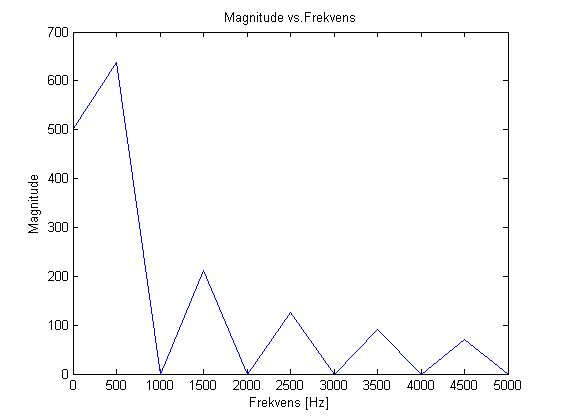
\includegraphics[width= 1\textwidth]{Figurer/oppg4_plot.png}
       \caption{Målt Magnitude plottet mot frekvens}\label{fig:oppg4_plot}
  \end{center}
\end{figure}

Plottet kan sees i Figur \ref{fig:oppg4_plot}. Merk at Frekvens = 0 betyr DC verdien på signalet og at magniuden på dette systemet er lik \(b_{n}\) faktorene siden alle \(a_{n} = 0\).


\section{Oppgave 5: Rekonstruksjon av et firkantsignal}
\jf{5.a}
\begin{figure}
  \begin{center}
      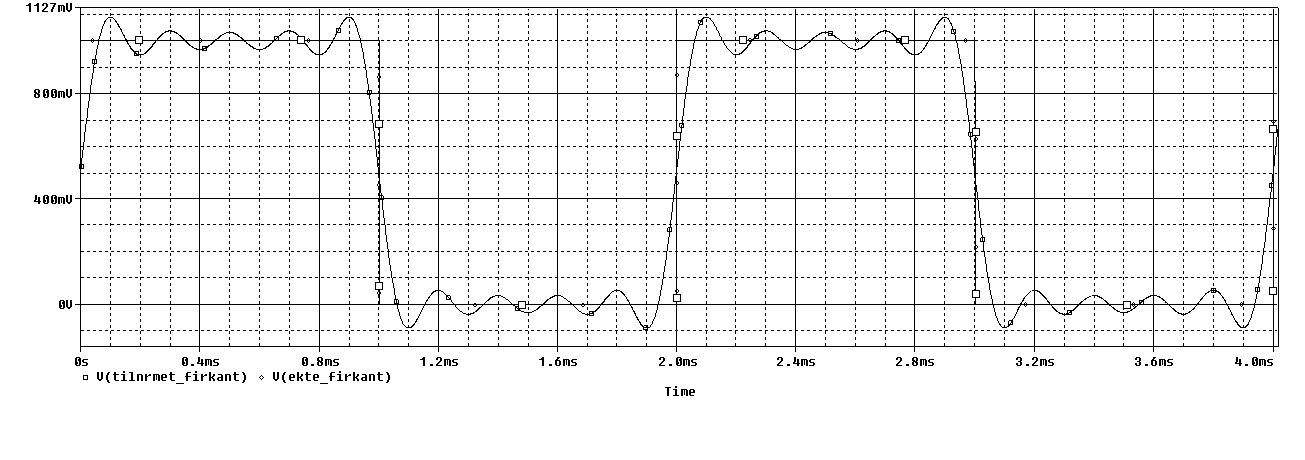
\includegraphics[width= 1\textwidth]{Figurer/oppgg5_A_vs_tid.PNG}
       \caption{Ekte firkant og Tilnærmet firkant satt i samme plott}\label{fig:oppg5a}
  \end{center}
\end{figure}



\section{Oppgave 6: Studie av spekteret til et firkantsignal når periodetiden
øker}
\jf{6.a}
\begin{figure}
  \begin{center}
      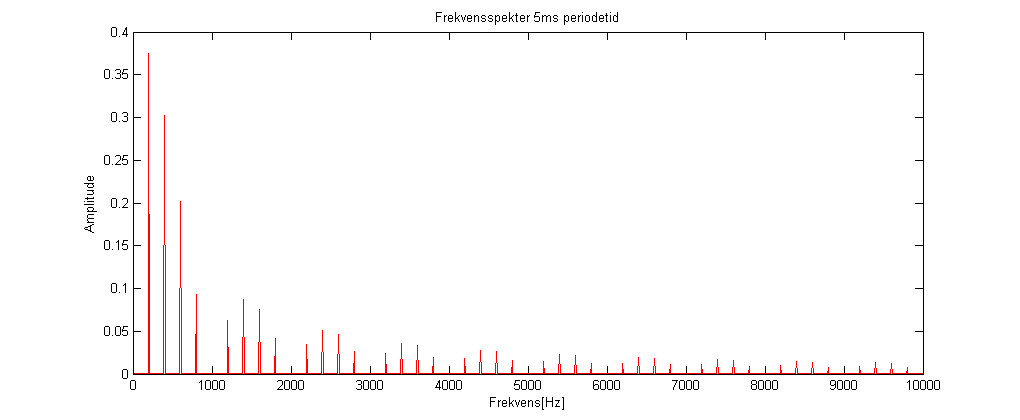
\includegraphics[width= 1\textwidth]{Figurer/oppg6_5ms.png}
       \caption{Fourierspekter av Firkantsignal. Pulsbredde 1ms , periodetid 5ms}\label{fig:oppg6_5ms}
  \end{center}
\end{figure}
\begin{figure}
  \begin{center}
      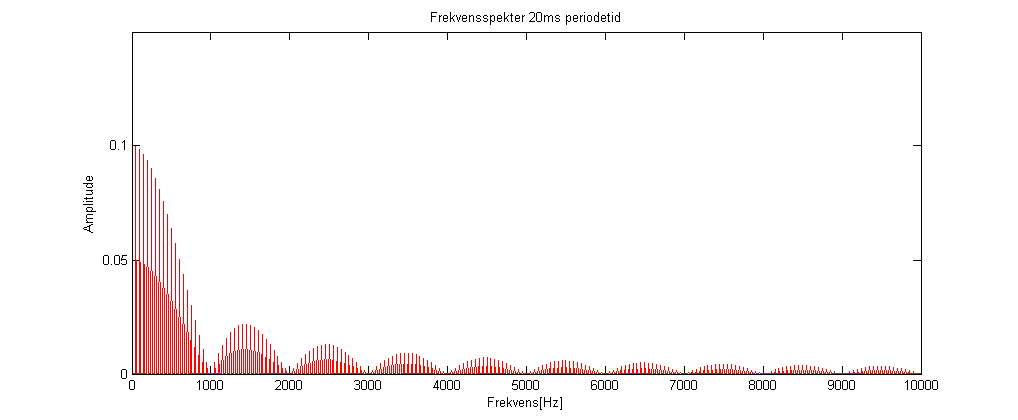
\includegraphics[width= 1\textwidth]{Figurer/oppg6_20ms.png}
       \caption{Fourierspekter av Firkantsignal. Pulsbredde 1ms , periodetid 20ms}\label{fig:oppg6_20ms}
  \end{center}
\end{figure}
\begin{figure}
  \begin{center}
      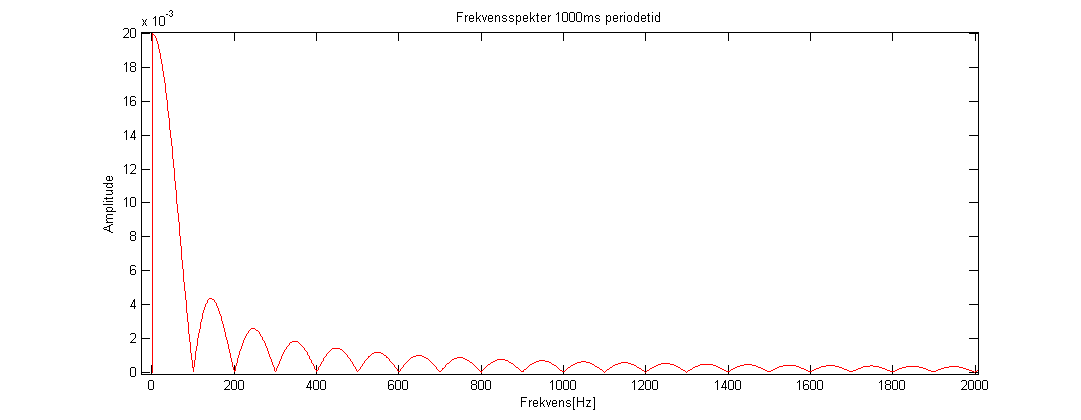
\includegraphics[width= 1\textwidth]{Figurer/oppg6_1000ms.png}
       \caption{Fourierspekter av Firkantsignal. Pulsbredde 1ms , periodetid 1000ms}\label{fig:oppg6_1000ms}
  \end{center}
\end{figure}

I Figur \ref{fig:oppg6_5ms} har firkantpulsene med bredde \(1\)ms en periodetid på \(5\)ms Vi ser at Frekvenspekteret har klare diskrete verdier for hvilke frekvenser som inngår i signalet. Vi ser amplituden på de forskjellige frekvenskomponentene avtar med en funksjon som likner en sinus cardinal funksjon

I Figur \ref{fig:oppg6_20ms} er periodetiden økt til 20ms. Vi ser at de diskrete verdiene ligger tettere en de gjorde i det forrige plottet og omhilningsfunksjonen som liknet sinc er enda tydeligere

I Figur \ref{fig:oppg6_1000ms} er periodetiden satt til 1000ms. Med oppløsningen vi har på analysen, oppfattes nå frekvensspekteret som kontinuerlig, og vi ser tydelig en sinc liknende funksjon

Vi ser at Amplituden til hver av frekvensene avtar etterhvert som signalet består av tettere komponenter 
\jf{6.b}

Vi ser at når periodetiden går mot uendelig og pulsbredden forblir den samme, kan man anse signalet som en enkelt puls. Som vi har sett i forelesning, får man ved Fourier Integral Analyse da en sinus kardinal funksjon for frekvensspekteret. 
\section{Oppgave 7: Studie av spekteret til en firkantpuls som har avtakende
pulsbredde}
\jf{7.a}
\begin{table}[H]
  \centering
  \begin{tabular}{r c}
    \toprule
    Pulsbredde [\unit{\textmu s}] & Båndbredde [kHz]\\
    \midrule
    $ 1000 $ & $1$\\
    $ 100  $ & $10$\\
    $ 30   $ & $32.4$\\
    $ 10   $ & $91.5$\\
    $ 3    $ & $252$\\
    $ 1    $ & $480$\\
    \bottomrule
    \end{tabular}
  \caption{Sammenheng mellom pulsbredde og båndbredde for en firkantpuls med
  periode på 1000 ms}
  \label{tab:bandwidth}
\end{table}
Se Tabell \ref{tab:bandwidth} for pulsbredde og Frekvensspekterets båndbredde.
\jf{7.b}
Se Figur \ref{fig:oppg7_plot} for plot av Tabell \ref{tab:bandwidth}
\begin{figure}
  \begin{center}
      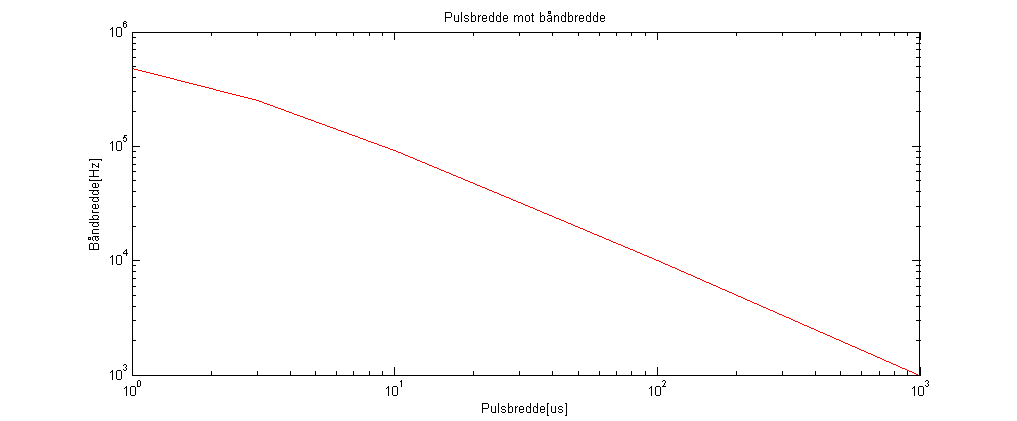
\includegraphics[width= 1\textwidth]{Figurer/oppg7_plot.png}
       \caption{Pulsens bredde plottet mot Frekvensspekteret båndbredde}\label{fig:oppg7_plot}
  \end{center}
\end{figure}
\jf{7.c}

\begin{figure}
  \begin{center}
      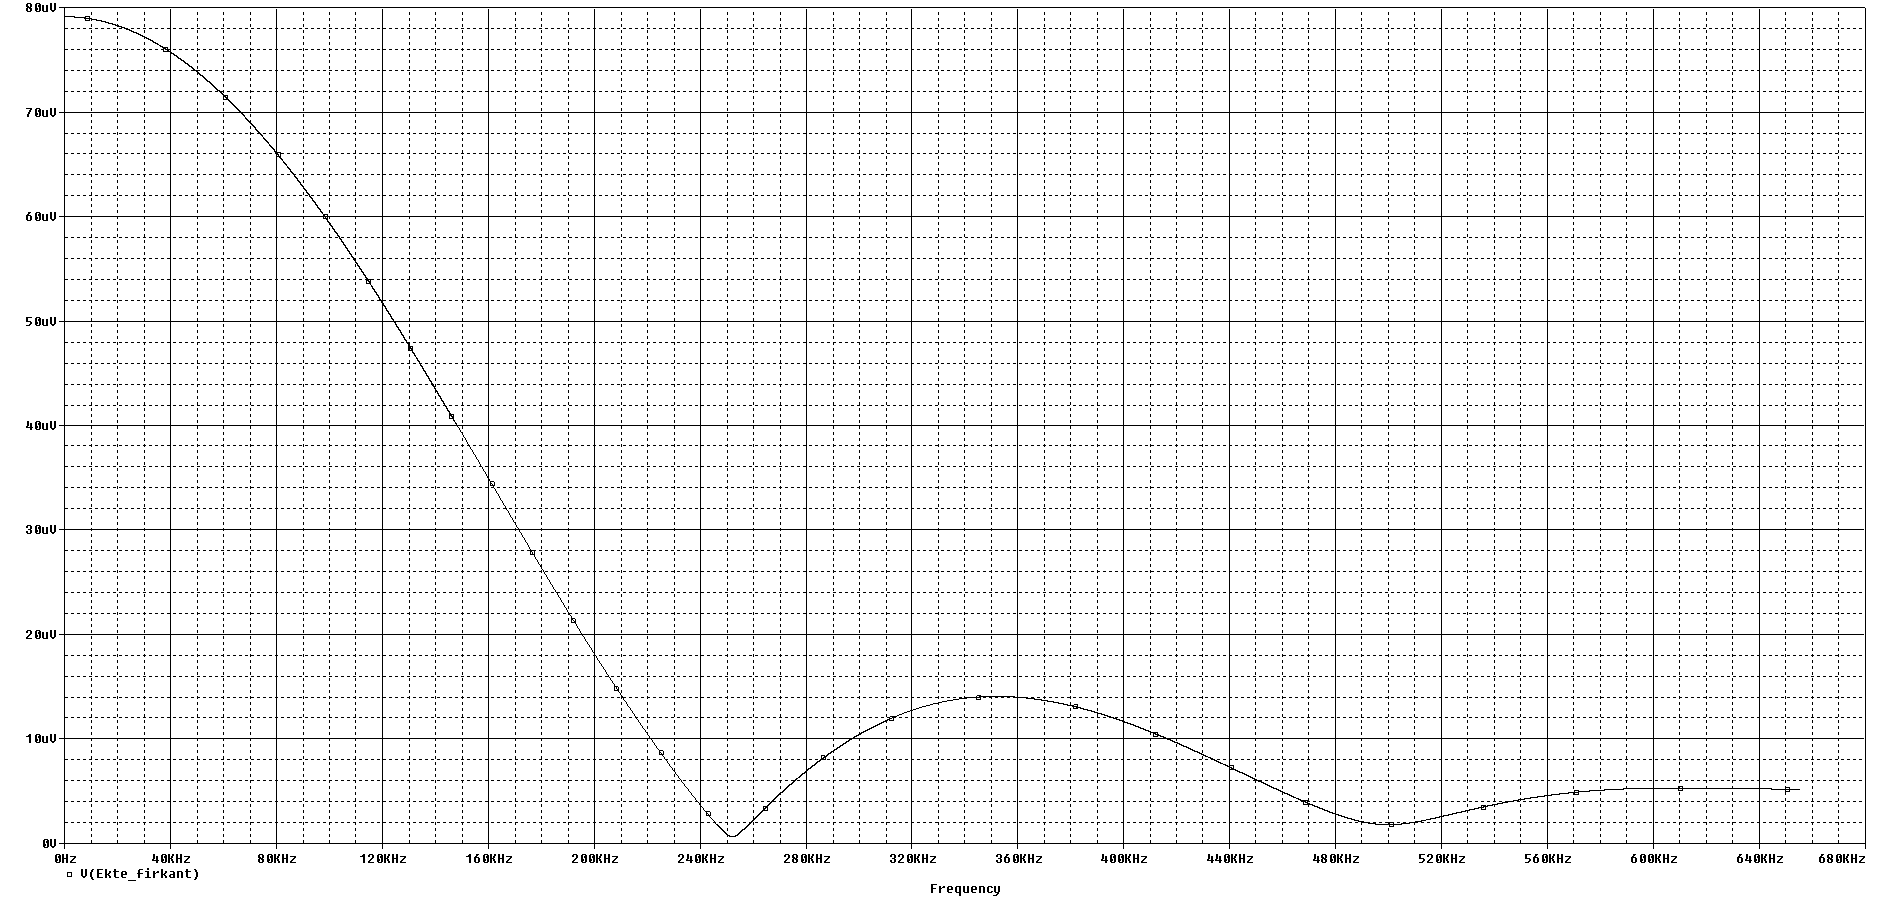
\includegraphics[width= 1\textwidth]{Figurer/oppg7_3us.png}
       \caption{Frekvensspekteret til en firkantpuls med bredde 3us og periode 1000ms}\label{fig:oppg7_3us}
  \end{center}
\end{figure}
\begin{figure}
  \begin{center}
      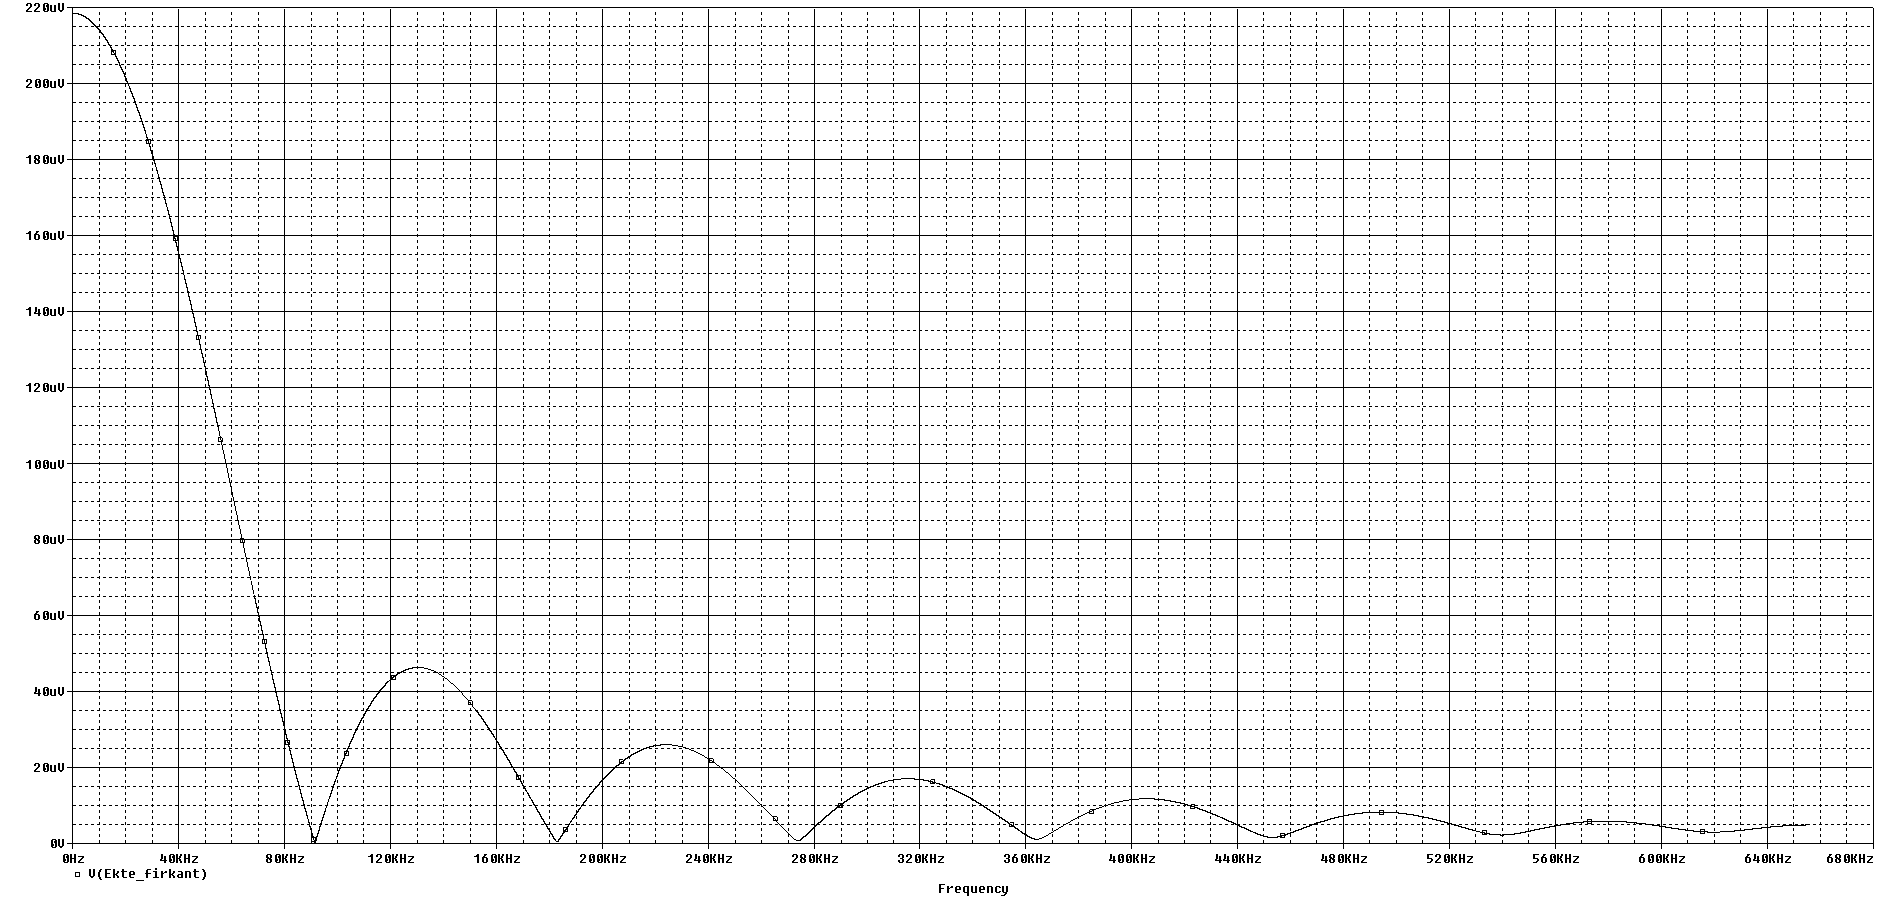
\includegraphics[width= 1\textwidth]{Figurer/oppg7_10us.png}
       \caption{Frekvensspekteret til en firkantpuls med bredde 10us og periode 1000ms}\label{fig:oppg7_10us}
  \end{center}
\end{figure}

Se plot for 3us puls i Figur \ref{fig:oppg7_3us} og 10us i Figur \ref{fig:oppg7_10us}

\jf{7.d}
Vi ser at når pulsbredden avtar, brer hovedloben til frekvensspekteret seg ut slim man kan se i Figur \ref{fig:oppg7_plot}. Vi kan anta at når pulsen blir uendelig smal, vil båndbredden bli uendelig stor, og frekvensspekteret til den smale pulsen vil bestå av av alle frekvenser med like stor amplitude.

\section{Oppgave 8. Studie av frekvensspekteret til en ekte sagtann}

\jf{8.a}
\begin{table}[H]
  \centering
  \begin{tabular}{l r p{1.7cm} p{1.9cm} p{1.9cm} p{1.5cm}}
    \toprule
    & $n$ & $b_n$ Firkant \par [mV] & $b_n$ Sagtann1 \par [mV]
    & $b_n$ Sagtann2 \par [mV] & Frekvens \par [kHz] \\
    \midrule
     DC verdi & 0 & 500 & 500.3 & 499.9 & 0\\
     Grunntone & 1 & 636.6 & 318.3 & 318.3 & 0.5\\
     2-Harmoniske & 2 & 0 & 159.2 & 158.6 & 1\\
     3-Harmoniske & 3 & 211.7 & 105.4 & 105.8 & 1.5\\
     4-Harmoniske & 4 & 0 & 79.41 & 79.31 & 2\\
     5-Harmoniske & 5 & 126.4 & 63.37 & 63.66 & 2.5\\
     6-Harmoniske & 6 & 0 & 53.02 & 52.85 & 3\\
     7-Harmoniske & 7 & 90.16 & 45.47 & 45.4 & 3.5\\
     8-Harmoniske & 8 & 0 & 39.66 & 39.58 & 4\\
     9-Harmoniske & 9 & 70.73 & 35.37 & 35.31 & 4.5\\
     10-Harmoniske & 10 & 0 & 31.79 & 31.81 & 5\\
    \bottomrule
  \end{tabular}
  \caption{Sammenheng mellom frekvenskomponentene til et firkant- og sagtannsignal}
  \label{tab:komponenter_sagtann}
\end{table}

\jf{8.b}
Som tabell \ref{tab:komponenter_sagtann} viser så er verdiene målt i frekvenspekteret tilnærmet lik for de to sagtann signalene. Dersom vi sammenligner med verdiene vi målte fra firkantsignalet ser vi at sagtannpulsene ikke får verdien 0 der \(n\) er et partall. Dette kommer av forskjellen mellom sagtannsignalet og firkantsignalet.

\section{Oppgave 9. Studie av tilnærmingsfunksjon for en ekte sagtann}
\jf{9.a}
\begin{figure}
  \begin{center}
      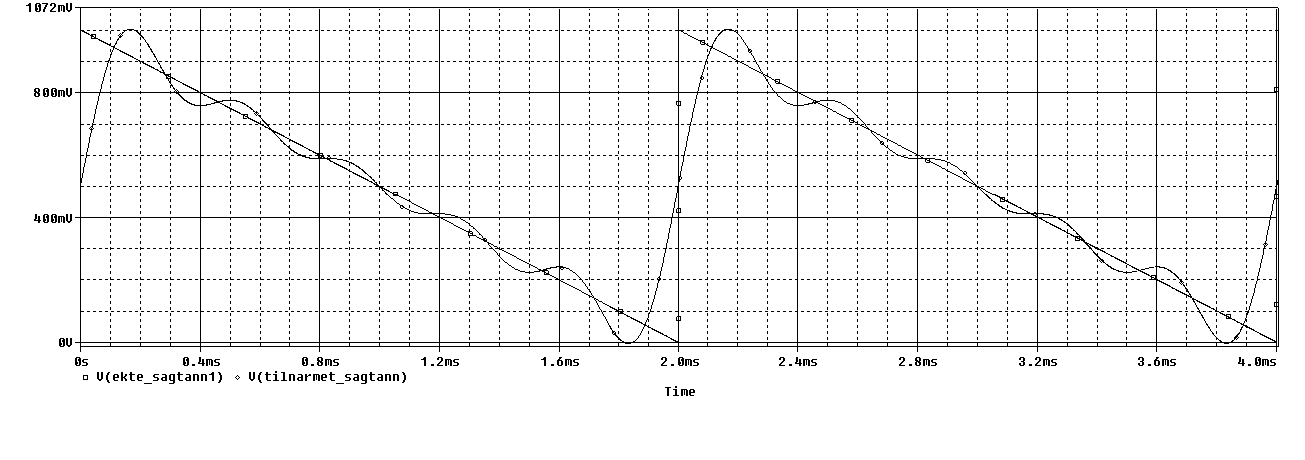
\includegraphics[width= 1\textwidth]{Figurer/oppg9a_sagtann.PNG}
       \caption{Her ser vi tilnærmet sagtann og ekte sagtann1 plottet sammen mot tid}\label{fig:oppg9a_sagtann}
  \end{center}
\end{figure}

Figur \ref{fig:oppg9a_sagtann} viser vårt tilnærmet sagtann signal plottet sammen med ekte sagtann1 over to perioder.

\section{Oppgave 10. Studie av fase for sagtannsignal}
\jf{10.a}
Frekvenskomponenter som måtte fasevendes 180 grader:

Vi fant ut at dersom vi fasevendet alle sinusgeneratorene så tilnærmet sagtann best ut i forhold til ekte sagtann2. Dette gir mening siden vi kunne se at ekte sagtann1 og ekte sagtann2 var 180 grader faseforskjøvet i forhold til hverandre.

\jf{10.b}
\begin{figure}
  \begin{center}
      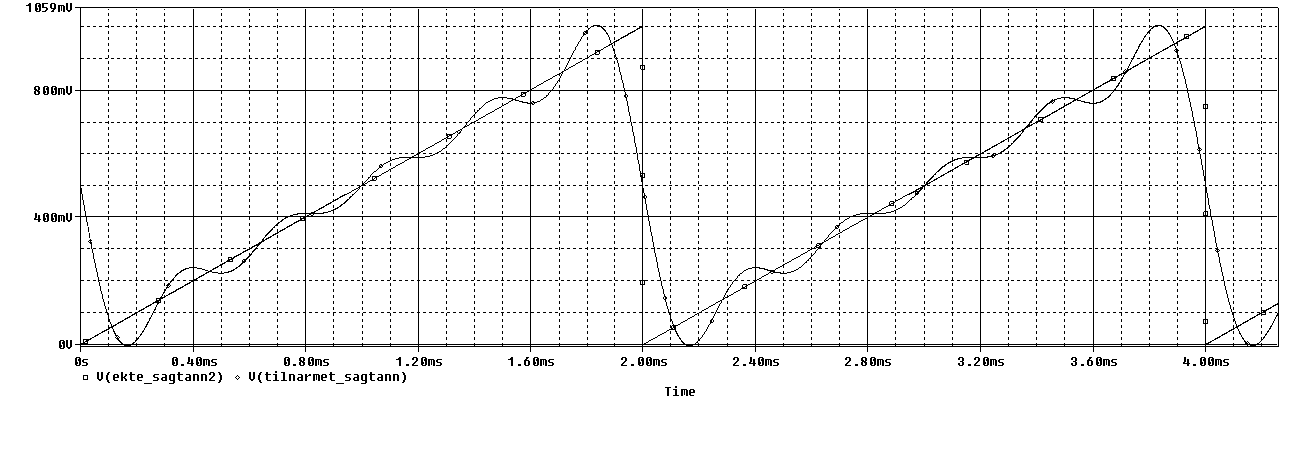
\includegraphics[width= 1\textwidth]{Figurer/oppg10b_sagtann_fase.PNG}
       \caption{Tilnærmet sagtann og ekte sagtann2 plottet sammen mot tid. Der alle sinusgeneratorene er faseforskjøvet med 180grader.}\label{fig:oppg10b_sagtann_fase}
  \end{center}
\end{figure}

Figur \ref{fig:oppg10b_sagtann_fase} viser plott av tilnærmet sagtann og ekte sagtann2 plottet sammen over to perioder. Vi kan se at den tilnærmede signalet passer meget godt med det ekte signalet.
\end{document}
